\section{反三角函数}

\begin{definition}[反三角函数]
    \begin{minipage}{0.45\textwidth}
        设$y=\arcsin x$，当且仅当$\sin y = x$且$-\frac{\pi}{2} \leq y \leq \frac{\pi}{2}$。

        设$y=\arccos x$，当且仅当$\cos y = x$且$0 \leq y \leq \pi$。

        设$y=\arctan x$，当且仅当$\tan y = x$且$-\frac{\pi}{2} < y < \frac{\pi}{2}$。

        反三角函数具有单值性，即不会出现像三角函数一样的周期。因为 $x \in [-1,1]$，不能对应很多个 $y$ 值。
    \end{minipage}
    \hfill
    \begin{minipage}{0.5\textwidth}
        % arcsin
        % AXIS ENVIRONMENT: arcsin, arccos, arctan
        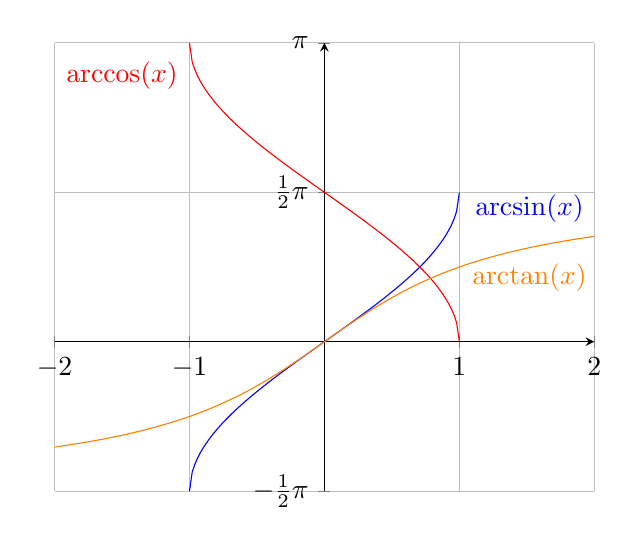
\begin{tikzpicture}
            \begin{axis}[enlargelimits=false,
                    axis lines=middle,
                    xtick={-2,-1,0,1,2},
                    ytick={-1.570780, 1.570780, 3.14159},
                    yticklabels={$-\frac{1}{2}\pi$,$\frac{1}{2}\pi$,$\pi$},
                    grid=major,
                    samples=100
                ]

                % arcsin
                \addplot[domain=-1:1,no marks,blue] {rad(asin(x))};
                \node at (axis cs:1.52,1.4){\color{blue}$\arcsin(x)$};

                % arccos
                \addplot[domain=-1:1,no marks,red] {rad(acos(x))};
                \node at (axis cs:-1.5,2.8){\color{red}$\arccos(x)$};

                % arctan
                \addplot[domain=-2:2,no marks,orange] {rad(atan(x))};
                \node at (axis cs:1.52,.67){\color{orange}$\arctan(x)$};

            \end{axis}
        \end{tikzpicture}
    \end{minipage}
\end{definition}

\begin{theorem}[$arcsinx$ 的性质]
    \begin{itemize}
        \item 首先是一个奇函数，则可以 $arcsin(-\frac{1}{2}) = -arcsin(\frac{1}{2}) = -\frac{\pi}{6}$
        \item 显然是有界的，而且单调递增。
        \item
    \end{itemize}
\end{theorem}

\begin{theorem}[两个重要结论]
    \begin{itemize}
        \item $\arcsin x+\arccos x=\frac{\pi}{2}, x \in[-1,1]$.
        \item $\arccos (-x)=\pi-\arccos x, x \in[-1,1]$.
    \end{itemize}
\end{theorem}

\begin{definition}[反正切与反余切]

\end{definition}
